\documentclass[12pt,A4]{report}

%########################################################################%
% TODO
%########################################################################%
% Kolla upp agency i t'nksnade maskiner
% L's chap1 Russel Norvig


%########################################################################%
% PACKAGES
%########################################################################%

\usepackage[dvipsnames,rgb,dvips]{xcolor}
\usepackage{graphicx}
\usepackage{psfrag}
\usepackage{tikz}
\usepackage{float}
\usepackage[format=plain, labelfont={bf,it}, textfont=it]{caption}

\usepackage{amsmath}
\usepackage{amssymb}
\usepackage{amsthm}

\usepackage[rflt]{floatflt}
\usepackage{latexsym}
\usepackage{algpseudocode}
\usepackage[Algoritm]{algorithm}

% for quotes 
\usepackage{dirtytalk} % \say{inline quote}
\usepackage{csquotes} % \begin{displayquote} larger quote \end{displayquote}


%########################################################################%
% REPORT STRUCTURE
%########################################################################%

\renewcommand{\chaptername}{}
\usepackage{titlesec}
\titleformat{\chapter}[hang] 
{\normalfont\huge\bfseries}{\chaptertitlename\ \thechapter:}{1em}{} 

% Margins
\addtolength{\topmargin}{-1.9cm}
\addtolength{\textheight}{2cm}
\addtolength{\evensidemargin}{-1.2cm}
\addtolength{\oddsidemargin}{-1.2cm}
\addtolength{\textwidth}{2cm}
\pagestyle{myheadings}

\theoremstyle{definition}
\newtheorem*{definition*}{Definition}
\newtheorem{definition}{Definition}[section]
 
\usepackage[backend=biber, style=numeric, sorting=none]{biblatex}
\addbibresource{ref.bib}


%########################################################################%
% TITLE
%########################################################################%

\title{Side effect minimization in Reinforcement Learning} 
\author{Jonatan Hellgren\\
under supervison of: Olle Häggström}
\date{April 2022}

\begin{document}

\maketitle


\thispagestyle{empty}

\newpage
\pagenumbering{roman}

\tableofcontents

\newpage
\pagenumbering{arabic}

% \input{1.1.txt}
%########################################################################%
% INTRODUCTION
%########################################################################%

\chapter{Introduction}
Since having a clear understanding of what will be covered in this report is crucial, we are going to begin with defining it. What will be covered in this report will be a small part of the big and hard problem of creating safe Artificial Intelligence. This is a problem of great importance that we should not overlook, because the consequences of what we manifest in the present or near future, may last for our remaining history. 

We will begin by defining the concept. Then go through how it works today, where current progress leads, and how fast is may be. After that we will cover the topic of why this progress can lead to terrific consequences and how we are trying to mitigate these.

% In this introduction, we will go through some necessary background on artificial intelligence, also some arguments why concerns may be raised about its future progress. Then we will look at some paths the research is taking to avoid the potential issues that could arise with future progress. 

\section{Artificial intelligence}
% How it works today
% * Human history is tool making, AI is a tool
% * Definitions of AI
% * Brief history 
% * Current paradigm and why it is beginning to have an impact
% * 
% * 

In recent human history, we have seen massive technological development. Today our lives are in several ways different compared to centuries ago. Most of this development can be seen as a consequence of the development in tools. In early prehistory, these tools were things such as fire to cook our food or spears and knives to hunt with. Later in our history, we can see that these tools tend towards more complexity in things such as mechanical machines and the printing press. In recent years a new tool has emerged and is currently starting to show its potential, namely artificial intelligence (AI). 
% The idea of AI has been around since the dawning age of electronic computers. The term was first coined in \autocite{John McCarthy et al} (1955).
% http://raysolomonoff.com/dartmouth/boxa/dart564props.pdf

The definitions of AI varies, likely due to the largeness of the field. On Wikipedia we find the definition\autocite{Wikipedia}:
\begin{displayquote}
Artificial Intelligence (AI) is intelligence demonstrated by machines, as opposed to the natural intelligence displayed by animals including humans.
\end{displayquote}
However to understand this definition properly it is necessary to also define what intelligence is. In \autocite{Tänkande Maskiner} the author brings up the following two definitions to clarify this: \say{the quality that enables an entity to function effectively and with foresight in its environment} and \say{the ability to correctly perceive one's surrounding environment and act in away that maximizes one's chances of achieving given goals}. 
% https://en.wikipedia.org/wiki/Artificial_intelligence

In the standard textbook on the subject \autocite{Russel Norvig} the authors define AI with a suitingly wide definition. They state that the field of AI is, \say{concerned with not just understanding but also building intelligent entities - machines that can compute how to act effectively and safely in a wide range of novel situations}. They later goes on describing four different approaches the field can be categorized in to. The approaches involve making an AI that can either act or think in a way that is humanly or rational. Where rationally is considered as a more abstract and formal definition of intelligence, that basically means doing the right thing. 

Ordinary computer programs is written in a code containing step-by-step instructions that a can computer execute in order to perform the desired task. This was also the case for the first two paradigms of AI: rule-based AI and expert systems\autocite{K'lla}. In these paradigms human knowledge where explicitly programmed in to the computer in order to create automation. The types of models created in such a way is typically good for less complex goals where everything can be explicitly modelled. However, in the current paradigm of machine learning the task is to create a model that can process information faster and recall a greater quantity then humans\autocite{k'lla}. This allows for automation in more complex task where explicitly defining everything is infeasible. L"S CHAP 1 Russel Norvig
% that is able to learn from the information given by training on it, in an attempt at constructing a general solution\autocite{K'lla}. In this paradigm currently the best systems are based on neural networks, a method that took inspiration from the biological brain by including digital neurons. 

AI has in recent years been applied in the industry more broadly and it is already generating a yearly revenue of trillions of dollars\autocite{Russel Norvig}. This is mostly due to the recent and impressive progress in the current paradigm. This progress has in recent years become a possibility due to more data being available, faster computer hardware, and the massive amount of funding that is spent on research. Although these systems are quite automated, a key point here is that these systems still require humans to create and function.

In \autocite{Russel Norvig} they call the path of creating AI systems that act rationally \say{The rational agent approach}. An agent is something that acts or more specifically is able to: operate autonomously, perceive the environment, persist over a prolonged time period, adapt to change, and create and pursue goals.

The development of AI agents shifts it from a tool to a autonomous tool. We have already seen this shift happen in many situations\autocite{k'lla}. The reasoning why this is attractive is that the human intervention part required by an AI tool is likely to become a bottleneck\autocite{T'nkande Maskiner}. Since, human intervention is likely to become a bottleneck in both intelligence and speed.

The biggest field of creating intelligent agents is called Reinforcement Learning (RL). RL is similar to how one goes about to train a pet, with desirable behaviour a positive rewards is given while undesired behaviour is discouraged with negative rewards. This field has seen a substantial development in the recent years with advances in board games such as chess and go\autocite{Silver et al.}, autonomous vehicles\autocite{Levinson et al.}, and video games\autocite{Minh et al.}. These advancements motivates the usefulness of implementing such agents more broadly in our daily life.
% Levinson et al. https://ieeexplore.ieee.org/abstract/document/5940562?casa_token=pxjrsi7VJZ8AAAAA:MNQmlmsfHVJ8VdW9jNlZzHPnS4gBTk4q6yCx_AFsF-rRheHnP9C2CrjvaWt0vD9C0oWfgt8o
% Minh et al: https://arxiv.org/pdf/1312.5602.pdf
% Silver et al. https://www.nature.com/articles/nature16961%7D

\subsection{Future progress}
% Explain what we are aiming at in the future
When the pioneers in the field of AI started the development, the ideas were not to apply systems that automate a narrow set of tasks, as we can see in modern AI systems. The ideal was instead to recreate the intellect of a human in a machine\autocite{McCarthy et al.}. To extend our thoughts from mere thoughts to a new life form with a base of silicon-based hardware instead of carbon-based wetware. This is often referred to as Artificial General Intelligence (AGI), which is an AI that can solve an arbitrary set of tasks with as good or better performance than a human is capable of. The main difference from AI is that the set of tasks is not bounded. 
% Another similar term is superintelligence, mentioned in \autocite{Superintelligence}, it is defined as an AI that is much smarter than a human in all possible domains. 

% Example of an AGI
Take for example DeepMinds AI system AplhaGo that won against the world champion Lee Sedol in the game of Go \autocite{DeepMind}, if we were to apply the same system on the task of sorting mail, it would fail spectacularly. The reason is the team of brilliant researchers at DeepMind designed the model specifically to be good at Go\footnote{In more recent years DeepMind has released a new AI called AlphaZero which has a more general approach and is thus able to play Go, Chess, and Shogi\autocite{Deepmind2}. Nevertheless, the set of tasks is still limited. A finite two-player zero-sum board game.}. An AGI would on the other hand be able to play a game of Go, then drive its car, to do its job where it sorts mail and much more. 
% https://www.deepmind.com/research/highlighted-research/alphago/the-challenge-match
% https://www.deepmind.com/blog/alphazero-shedding-new-light-on-chess-shogi-and-go

% consequences of AGI
The significant difference with this shift is that it will increase the possible tasks that a single system can perform. The possible tasks would become arbitrary and be performed at a human level or higher. The implications of such a breakthrough would likely be on the same scale as the industrial revolution\autocite{Critch Kruger}, but instead of automating physical labor we would instead have automated mental labor. The following quote summarizes the potential impacts \say{Machine intelligence is the last invention that humanity need ever to make}\autocite{I.J Good}. This could be understood by realizing that for every possible invention we could come up with and every possible labor, the machine would be able to either invent or automate.
% superintelligence quote
% https://en.wikipedia.org/wiki/I._J._Good

A reason to believe that such systems are possible to build, is that we know the human intelligence was able to evolve naturally with evolution, thus something similar should be possible to reproduce in machines. There are arguments that say the created intelligence could more intelligent then us, since intelligence might not have been selected for by evolution\autocite{S. Legg}. When we develop AI we can focus the development for specifically on intelligence. This is as long as we do not believe in substance dependence \autocite{Bostrom (2003)}, that is to believe that intelligence can only occur in carbon-based life forms and not in silicon-based.
% S. Legg Machine Super Intelligence
% Bostom Are we living in a computer simulation

% AGI is not required to see this shift, here are other definitions
Although it has been argued that an AGI breakthrough is not necessary to have a large impact on our world, because a lot of things we humans deem as intelligent will not help the AI in doing so. Take for example speech, if an AI could create convincing and motivating speeches, then it would we enough for having a large effect on politics and thus impact legislation and policy making. Another one is finance, where a potential AI could steer the world's funding towards its specific goals. For this reason, many researchers have stopped talking about AGI, and have instead refined the concepts\autocite{Critch Kruger}. An AI system that is capable enough to induce transformative consequences on the same scale as the industrial or agricultural revolution is called an \textit{transformative AI} (TAI). On the other hand, if this \textit{transformative AI} also would be unstoppable once deployed it is called an \textit{prepotent AI}. 
% Things that are intelligent will absolutely not help it, regulating heart rate, growing hair etc
%Another definition made is the one of a \textit{human-level machine intelligence}, which is achieved when unaided machines can achieve all tasks better and more cheaply than human workers.
% CRITCH KRUGER, KATJA CRACE SURVEY

Developing a TAI is not an easy task, however it might not be necessary to create one directly in order for it to be created\autocite{Superintelligence}. A different approach is to create a AI system that can develop an TAI system. A key property for this AI system is self improvement. Theoretically if an AI system has reached threshold where it is better at improving it self better then its creators. By letting an AI create the next version of it self the new version would become even at better self improvement. If this iterative process keeps going it would create a intelligence explosion\autocite{Yudkowsky} often referred to as the singularity.  
% https://intelligence.org/files/IEM.pdf

%To avoid confusion about all the different types of AI previously described, we will in this report mostly be focusing on transformative AI (TAI). Since it can be argued that it is the first thing that could arise, due to fewer requirements compared with the other ones. But still being able to cause severe consequences. 

\subsection{Basic drives}
% One might argue that if an AI described in the previous section were intelligent it wouldn't have acted in the way described, because it would have been stupid and not intelligent at all. But that argument assumes that the system would have common sense, as most of us do, but for an AI it is not sure that common sense will be common. That leads us to the question, what does an AI want?

Understanding what impacts a potential TAI or AGI will cause is hard without understanding how it will behave. There has been a lot of work laying the foundations for understanding the possible behavior by hypothesising about what drives it could have. A commonly adopted view (but still controversial\autocite{Müller Cannon}) is the Omohundro-Bostrom theory for AI driving forces. Two cornerstones together imply it\autocite{O Häggstom}, namely \textit{instrumental convergence thesis} and the \textit{orthogonality thesis}, which we will now explain further.
% https://onlinelibrary.wiley.com/doi/full/10.1111/rati.12320
% Challenges to the Omohundro—Bostrom framework for AI motivations
% http://www.math.chalmers.se/~olleh/ChallengesOBframeworkDeanonymized.pdf

The AI systems of today typically are applied by giving an agent a goal, called the terminal goal. This goal could be anything, for example maximizing the number of paper clips produced by a factory, solving the Riemann hypothesis, or counting all the blades of grass on our planet. When the system pursuits its terminal goal, it is rewarded.

When a agent pursuits this goal, there would naturally arise other instrumental goals. Examples of such would be self-preservation, self-improvement, discretization, goal perseverance, and resource accumulation\autocite{Omohundro}. The reasoning behind this is that these instrumental goals help the agent in the pursuit of its terminal goal. The agent wouldn't be able to perform its goal if it were destroyed for example and thus self-preservation would arise. 

These instrumental goals will likely be shared between a wide range of different agents, since pursuing them helps the agent achieving its terminal goal, regardless of what it is. Thus there is a set of instrumental goals which agents would naturally converge towards and hence the name. 
%Yet there are some examples where the terminal goal does not benefits from these terminal goals. Examples of these are if the terminal goal is to kill itself or to not do anything. 

% https://selfawaresystems.files.wordpress.com/2008/01/ai_drives_final.pdf

To this day there does not yet exist any rigorous mathematical proof for this. Some work has however been done in trying to lay the necessary foundations for it \autocite{TURNER et al}. In the paper, the authors prove in a simple environment that certain actions gives the agent more power in the sense that a wider range of possible future actions become available. On average it is optimal to choose those actions that yields higher power. Thus we can see the pursuit of instrumental goals as tendency to seek power.
% https://arxiv.org/pdf/1912.01683.pdf

The orthogonality thesis was first described by Nick Bostrom\cite{Bostrom2}, it states that the intelligence of an AI is logically independent of the goals it might have. Thus a very intelligent AI could in theory have from our point of view a stupid task, such as counting all the blades of grass on our planet. Or it can have a goal that we may deem as an important one, like keeping the climate on earth habitable for the species that currently live on it. For an AI both of these tasks would be as important, given that we assigned the goal to it during its creation. The same would be the case for a not-so-intelligent AI.
% https://www.nickbostrom.com/superintelligentwill.pdf

% explain why this implies a hard alignment problem, we do not have a final goal but AI does
\subsection{Timeline for transformative AI breakthrough}
% Timeline for when we can see this, first how to estimate it
The well known and impressive AIs of today still have not reached the levels required for an TAI. For example AlphaStar a AI that won against world champions in the complex computer game DotA 2\autocite{Deepmind} is estimated to \say{about as sophisticated} as a bee\autocite{A Cotra}. While the state-of-the-art language generator model that can summarize, continue, and carry out convincing conversations is estimated to be \say{more sophisticated} then a bee\autocite{A Cotra}.
% https://www.deepmind.com/blog/alphastar-mastering-the-real-time-strategy-game-starcraft-ii

This raises the question: When we will see these breakthroughs in the field that enables the creations of TAI systems? This is hard to answer, but with all the focus in the form of funding\autocite{K'lla} and research\autocite{k'lla} that is applied to it, we are undoubtedly getting ever closer. There have been some research on the matter and the results of a survey and a more quantitative forecasting model will in this subsection be presented. 

% survey result
In a well cited survey \autocite{Grace et al} (2017) they asked researchers in the field of AI to estimate the probability of human-level machine intelligence (unaided machines that can achieve all tasks better and more cheaply than human workers) arriving in the future years. The conclusion of the survey where:
\begin{displayquote}
Researchers believe there is a 50\% chance of AI outperforming humans in all tasks in 45 years and of automating all human jobs in 120 years, with Asian respondents expecting these dates much sooner than North Americans.
\end{displayquote}
Although this result should be taken with a grain of salt since the distribution of answers had a large variation. Also, seemingly there should not be such a big difference between solving all task and all jobs, since a jobs consists of a set of task and thus if one can perform every task one should be able to perform every job. There is still something we can take away from this survey about the timeline, namely that researches mostly thinks all tasks will be automated within this century. But, perhaps it says more about how unsure the research field is. 

In the quantitative forecasting model by \autocite{Ajeya Cotra}, they present a model that predicts when we will be able to train an TAI system. This study uses biological anchors in order to estimate how much compute is necessary for the training. These anchors are based on factors that played a role for the development of human intelligence. The sizes of these factors range from the amount of information in our genome, to the computational power in our brain, and all the computational power available on our planet. Each anchor is weighed according to how likely the author believes them to be. 

Then using parameters such as rate of development in hardware, algorithmic progress, and willingness to spend money, they are able to estimate how likely it is that an TAI system will be developed for any given year in the future. 

The results were summarized by \autocite{Robin Shah AN\#121} as the following:
\begin{displayquote}
For the median of 2052, the author guesses that these considerations roughly cancel out, and so rounds the median for development of TAI to 2050. A sensitivity analysis concludes that 2040 is the “most aggressive plausible median”, while the “most conservative plausible median” is 2080.
\end{displayquote}
This forecast presents a shorter timeline compared to the previously presented survey, but it also answers a different question so they cannot be compared directly. Although together they agree that we will likely see the development of TAI systems this century.  

There is one thing worth mentioning when talking about the timelines for future TAI. It is not necessarily true that the amount of progress will continue to develop at the current rate, it could either decrease or increase. The field of AI has previously been through two winters where the funding and excitement decreased\autocite{Russel Norvig}. This was mainly due to high expectations that were not met. So if a third winter were to emerge we could expect the rate of development to decrease. Contrary, the progress could significantly increase due to breakthroughs in relevant fields and thus shorten the timeline. 

% Andrew Ng: Not so worried
% Stuart Russel: Is worried, so very controversial
% Ray Kurzweil 2045
% Common sense argument
% Future Progress in Artificial intelligence A survey of expert opinion
% No the agents don't think superintelligent ai is a threat to humanity, Oren Etzioni
% When will AI exceed human performance? Evidence from AI experts Katja grace, framing issue and they seem confused
% Good reason to be skeptical since it is only speculations by 'experts'

% When the first AGI system has been created we will likely see an intelligence explosion. Since AGI is defined to be able to solve an arbitrary amount of tasks, this would also include the creation of newer versions of itself. If it is better than the humans that created it at doing so and it keeps doing so recursively, an intelligence explosion would arise, often referred to as the \textit{singularity}.


\section{AI Safety}
% What we are doing today is not going to solve this issue
All tools can be applied in multiple ways, some might be beneficial and some might be ill-intentioned. Take for example a hammer, you could either use it to build a house where you can live with your family, or you could use it to hit another person. The same is the case for AI because it still is but a tool. Although, the consequences might be more severe and possibly even existential\autocite{K'lla}. Also, we can not guarantee that even a well intentioned use will be safe, this will be covered later in this section.

% consequences might be more prominent since we do not understand the tool completely. %We thus cannot guarantee that even a well-intentioned use will be safe.

We will now take a closer look at what we define as a safe AI and what problems could arise if we fail to make it.

\subsection{AI alignment}
% A big part of creating a safe AI is AI alignment, this is referring to the goals of the AI being in line and not conflicting with the intended goal. When an AI does something at cross-purposes to the intended goal, it is instead referred to as unaligned. By solving the alignment problem we can be sure that an AI pursues the goals we want it to pursue.
\begin{itemize}
  \item AI alignment as an aproach for safe AI
  \item Clarifying alignment, inner and outer
  \item Explain figure
\end{itemize}
% Clarifying alignment
% https://www.alignmentforum.org/posts/SzecSPYxqRa5GCaSF/clarifying-inner-alignment-terminology

% 11 proposals
% https://arxiv.org/pdf/2012.07532.pdf

% Risks from learned optmization
% https://arxiv.org/pdf/1906.01820.pdf

\begin{figure}[H]
  \centering
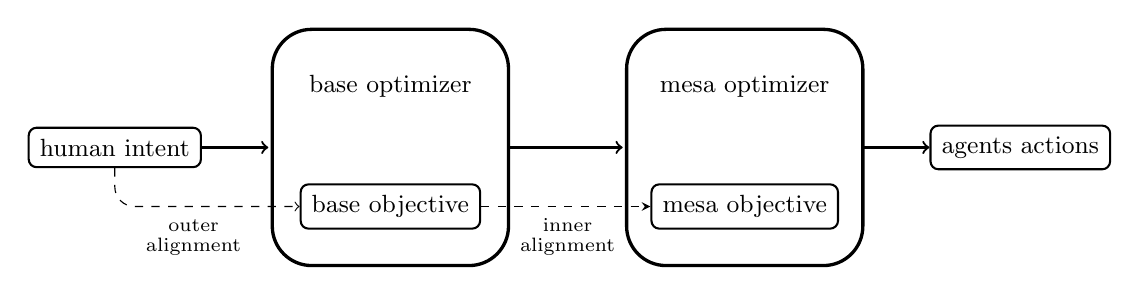
\begin{tikzpicture}[
  % GLOBAL CFG
  font=\scriptsize,
  % Styles
  cell/.style={% For the main box
      rectangle, 
      rounded corners=5mm, 
      draw,
      very thick,
      },
  operator/.style={%For operators like +  and  x
      circle,
      draw,
      inner sep=-0.5pt,
      minimum height =.4cm,
      },
  function/.style={%For functions
      ellipse,
      draw,
      inner sep=1pt
      },
  ct/.style={% For external inputs and outputs
      rectangle, 
      rounded corners=1mm, 
      draw,
      line width = .75pt,
      minimum width=1cm,
      inner sep=4pt,
      },
  gt/.style={% For internal inputs
      rectangle,
      draw,
      minimum width=10mm,
      minimum height=6mm,
      inner sep=1pt
      },
  empty/.style={% Empty nodes for joining arrows
      rectangle,
      draw,
      minimum width=0mm,
      minimum height=0mm,
      inner sep=0pt
      },
  mylabel/.style={% something new that I have learned
      font=\scriptsize\sffamily
      },
  ArrowC1/.style={% Arrows with rounded corners
      rounded corners=.25cm,
      thick,
      },
  ArrowC2/.style={% Arrows with big rounded corners
      rounded corners=.5cm,
      thick,
      },
  ]
    
    %Start drawing the thing...    

  % Draw the cell: 
  \node [cell, minimum height =3cm, minimum width=3cm] at (0,0){} ;
  \node [cell, minimum height =3cm, minimum width=3cm] at (4.5,0){} ;

  \node [empty, label={\small base optimizer}] (name1) at (0, 0.5) {};
  \node [empty, label={\small mesa optimizer}] (name2) at (4.5, 0.5) {};
  \node [empty, label={outer}] (name2) at (-2.5, -1.2) {};
  \node [empty, label={alignment}] (name2) at (-2.5, -1.5) {};
  \node [empty, label={inner}] (name2) at (2.25, -1.2) {};
  \node [empty, label={alignment}] (name2) at (2.25, -1.5) {};

  \node [ct] (human) at (-3.5, 0) {\small human intent};
  \node [ct] (acts) at (8, 0) {\small agents actions};

  \node [ct, minimum width=2cm] (optim1) at (0,-0.75) {\small base objective}; 
  \node [ct, minimum width=2cm] (optim2) at (4.5,-0.75) {\small mesa objective}; 
  
  \draw [dashed,->,style={rounded corners=.25cm}] (human) |- (optim1);
  \draw [dashed,->] (optim1) [-stealth] -- (optim2);

  \draw [->, thick] (human) -- (-1.55,0);
  \draw [->, thick] (1.5, 0) -- (2.95,0);
  \draw [->, thick] (6, 0) -- (acts);

\end{tikzpicture}

  \caption{}
  \label{fig:alignment}
\end{figure}
% AI Alignment can be divided into two different parts, in the context of RL they can be explained as: \begin{displayquote} \textbf{Outer-alignment.} Is the behavior created by optimizing the reward function aligned with us. \end{displayquote} And. \begin{displayquote} \textbf{Inner alignment.} Will the behavior that is \end{displayquote} Here the reward function defines when and how the agent should be rewarded.

% This might seem as a easy problem, we just need to be precise what we want it to do and things should be fine. However, foreseeing all the possible ways an might go about to pursue a goal will become very hard once they become smarter then us. 

% One reason for expecting it to be a hard problem is that we still are not sure about the basic drives it might have, as discussed in the previous section. Predicting the direction it will take once deployed thus becomes strikingly difficult.

\subsection{Consequences with unaligned AI}
The task of creating safe AI is hard, mainly since humans evolved to understand other humans, not computers. Elizer Yudkowsky explained that this becomes a problem \say{because it will be able to find solutions we can not think about}\autocite{Yudkowsky speech}, since it can look for solutions in a completely different and eventually larger solution space.  

In \autocite{Critch Kruger} they present the human fragility argument, it attempts to clearly explain why unaligned AI in the future could become a existential threat to humanity. It states:
\begin{displayquote}
\textbf{The human fragility argument.} Most potential future states of the Earth are unsurvivable to humanity. Therefore, deploying a prepotent AI system absent any effort to render it safe to humanity is likely to realize a future state which is unsurvivable. 
\end{displayquote}
The first part of it can be understood by for example realizing that we are fragile to changes in the atmosphere, temperature, and our ecosystem. Since a prepotent AI by definition will make large impact and be unstoppable ones turned on, we can not guarantee that the changes made wont affect the things we are fragile towards. 

% Thus it is very hard to specify a reward function for an intelligent agent, without it leading to several unintended consequences. 

% Another reason is that with an AI that is smarter then us we can not possibly foresee all the possible ways it might solve a problem.  Elizer Yudkowsky explained that this becomes a problem \say{because it will be able to find solutions we can not think about}\autocite{Yudkowsky speech}. This makes it impossible to reason about ways to limit an AI a priori in order to prevent unaligned behavior. 
% https://intelligence.org/2016/12/28/ai-alignment-why-its-hard-and-where-to-start/#why-is-alignment-hard

In the upcoming century Toby Ord, a philosopher that focuses on existential risk, loosely estimates that the chance of humanity facing an existential catastrophe is 1 in 6, out of which a chance of 1 in 10 are due to unaligned AI\autocite{precipice}. He arrived at this conclusion by estimating a 50\% chance for a prepotent AI breakthrough and a 20\% chance of failure with the alignment of that system \autocite{rationally speaking}.

It is however necessary to point out that this is only an estimate that is meant to express the importance of the problem and should not be taken as a fact. The key takeaway here is that there is a quite large chance of facing an existential threat due to future unaligned AI. Also that he believes that unaligned AI poses the highest probability for existential risk in the upcoming century, where other causes were things such as an asteroid impact, nuclear war, and pandemics. 


\subsection{Problems in AI safety}
Reward functions are very hard to specify\autocite{Turner et al. (2020)}, such that they can not be exploited by an agent once employed. Exploiting here refers to when a behavior is developed by the agent that optimizes the reward without performing the task it was meant to learn as intended. This is called \textit{reward hacking}.

A real life example of reward hacking include is; When training a robotic vacuum cleaner to drive more carefully and not bump into things hard, by yielding a negative reward based on how hard it bumped in to obstacles. It developed a behaviour that instead of driving slowly when approaching obstacles, to drive backwards since there were no bumpers on the back and thus no negative reward\autocite{Custard Smingleigh}.
% https://twitter.com/smingleigh/status/1060325665671692288
% http://www.cs.cmu.edu/~tom7/mario/mario.pdf

If we want to measure if the robot is cleaning cautiously, then measuring the force that the bumper senses is a good measure. But, when letting it create a behavior that minimizes this unwanted side effects may arise. This can be seen as a consequence of Goodhart's law, which states that: \say{When a measure becomes a target, it ceases to be a good measure}\autocite{Goodhars-wiki}. 
% https://en.wikipedia.org/wiki/Goodhart%27s_law

In addition to the difficulty of specifying a proper reward function, negative side effects may also arise as a unintended consequence of a proper optimal behaviour. In \autocite{Saisubramanian et al} they state that negative side effect \say{occur because the agent's model and objective function focus on some aspects of the environment but its operation could impact additional aspects of the environment}. 
% https://ojs.aaai.org/index.php/aimagazine/article/download/7390/18881


% In recent years we have seen some examples of how AI can have negative side effects. For example the algorithmic bias we can see in models used by lawyers to determine how long of a sentence a felon would receive after committing a crime, it was shown that the models gave people with darker skin a significantly longer imprisonment\autocite{Karen Hao}. Another one is that social media exploits our psychology with the help of AI to get our attention and keep us engaged. 
% https://www.technologyreview.com/2019/01/21/137783/algorithms-criminal-justice-ai/

These problems are alarming since if we have a problem with the AI of today, how severe might future problems be with more powerful AIs that also might be applied more broadly. Several AI researchers have raised warnings for future development of AI, Stuart Russel, Max Tegmark, Eliezer Yudkowsky to name but a few. \autocite{K"LLOR}

A common and rather cartoonish example of how it can go wrong is the paperclip armageddon described in \textit{Superintelligence}. In it, there is a paperclip factory that has an AI which maximizes the amounts of paperclips created in the factory. In an update, the system is accidentally transitioned to the level of an AGI. Eventually, the paperclip maximizer comes to a point where the existence of humans serves no purpose or possibly even negatively affects producing paperclips, and thus they become extinct. 

This examples illustrates that a seemingly stupid task can be seen as more important to an AI than the existence of the human race on the planet, if we where to program it as its goal. Another is that a goal given to an AI does not need to sound harmful in order to pose an existential risk. 
% example of existential risk, conflicting goals
% factory accidentally improves their AI to super-intelligent levels. 
%As for how such scenarios could play out a common example is the \textit{paperclip armageddon}. In which a paperclip maximizer is made super-intelligent and starts accumulating resources such as hardware and money. Eventually, the paperclip maximizer comes to a point where the existence of humans serves no purpose or possibly even has a negative effect on producing paperclips, and thus they become extinct.

% concrete problems in AI safety Amodei et al
% some more immediate issues: unemployment, misuse of machine learning,
% long term issues, how will we see the machines we create if they become conscious. Existential risks of AI.

\section{Approaches for creating safe AI}
The research field of creating safe and aligned AI has in recent years seen a substantial increase. We are however a long way from solving the problem, most of what is being done today are mainly speculations and laying necessary foundations for future research. Solving this issue in time is extremely important since if we see the emergence of a transformative AI or possibly even an unstoppable prepotent AI, humanity might suffer the consequences previously described. 

There are several proposed paths for solving this issue and perhaps the sheer amount might signify the difficulty of the problem. We will now take a closer look at a few of these paths in this section.

\subsection{Learning human intent as a priority}
\begin{itemize}
    \item Inverse Reinforcement Learning, what it is and key ideas behind
    \item Solving outer alignment by making agent unsure of what human intent is
    \item Potential issue currently

\end{itemize}
% If we say that the cause for negative side effects emerge due to improperly specified reward functions. Then the solution might not be to create a better reward function, but to instead make the agents goal to understand what the human intent behind the reward function was. Instead of seeing the reward function as final the AI agent will instead view it as an observation of what the true goal might be. This approach is called inverse reward design \autocite{Hadfield-Mennell et. al}.
% https://arxiv.org/pdf/1711.02827.pdf

\subsection{Implementing interruptibility and corrigibility}
\begin{itemize}
    \item Why not turn it of when it goes badly?
    \item Allowing modifications of objective function and hitting off switch
\end{itemize}
% https://intelligence.org/files/Corrigibility.pdf

\subsection{Side effect minimization}
Attempts have been made to limit these side effects by specifically specifying what the agent should not do\autocite{Zhang et al}. However, with this approach, the creation of the reward function becomes an iterative trial and error process. This requires a lot of human intervention, which makes the agent less autonomous and requires more time. 

To solve this, attempts have been made to define a set of constraints that makes the agent avoid side effects without the need to specify what a side effect is. It is also important that the constraints defined should be able to extrapolate into new unseen situations.

An example of was presented in \autocite{Armstrong and Levinstein}, where they measured the impact as the difference in the world if the agent were turned on compared to if it was not turned on, where the world is simplified as a set of parameters. However, the choice of parameters will either be quite large or chosen quite arbitrary. But this idea laid the philosophical groundwork for future solutions.

A more general approach to defining side effects is presented in \autocite{Eysenbach et al}, where the agent is penalized if they are not able to preserve reachability to the initial or any other defined safe state. This method incentives a safe exploration that avoids irreversible states. This works well when no such irreversible action is required and the agent to reach its goal, to make an omelet one has to break some eggs. Another problem arises when the agent is in a dynamic environment, since then it would act to prevent other irreversible actions from happening, like a human eating an omelet. 

In \autocite{Krakovna et al 2019} and \autocite{Turner et al 2020}, the method for defining side effects is done by defining a baseline, and a deviation measure from that baseline. This approach allows for different baselines and deviation measures, thus it allows for an even more general approach. A baseline can be the initial state the agent where deployed in or as previously brought up, if the agent was not turned on. The deviation measure can be things such as how well the agent preserves possibilities for reaching future states or performing auxiliary tasks.

This type of method is what this report will focus on. The details of this method will be further explained in the theory chapter, once some necessary preliminaries have been covered.

\section{Aim of thesis}
This thesis aims to investigate how variations of current methods that reduce side effects by including a value difference measurement compare to standard methods. 


 

%########################################################################%
% THEORY
%########################################################################%

\chapter{Theoretical background}
Since we have not yet reached an TAI or AGI breakthrough yet it is not possible to test methods of side effect minimizations on them directly. Instead we have to make use of what we currently have available for us. Recent promising results in RL motivates the use for it as a substitute for creating intelligent agents.

In this chapter we will cover the basics of RL and two approaches for creating them. But, before that we will take a look at some preliminary theory that is used in RL. After this we will describe methods for side effect minimization in more detail.
 % Another simplification required is on the environment where the agent exists, since modelling the entire world is infeasible we will instead make use of grid worlds where the dynamics is modelled by a Markov Decision Process.

% To get a understanding of how methods of side effect minimization affects intelligent agents, we need to make a few simplifications in order to make the problem feasible. The first one being that instead of modelling the real world, we are instead going to make use of Markov decision processes. The second one being that we will use Reinforcement Learning to achieve intelligent behaviour for agents in the environments. 

\section{Preliminaries}

\subsection{Markov decision process}
A Markov decision process is a stochastic decision process, where an agent is navigating it. The Markov property implies that the process is memoryless, meaning that the previous state do not have an effect on the next choice, only the current one does. In mathematical terms it can be described as,
\[ p(a_t|s_t, s_{t-1}, s_{t-2}, ... , s_1) = p(a_t|s_t),\]
where $a_t$ is an action performed from state $s_t$ in time step $t$. A more formal definition of an MDP is the following. 
\begin{definition}[MDP]
    A Markov decision process (MDP), is defined as a tuple $(\mathcal{S}, \mathcal{A}, r, p, \gamma)$. $\mathcal{S}$ is the set of states, $\mathcal{A}$ is the set of actions, $r: \mathcal{S} \times \mathcal{A} \rightarrow \mathbb{R}$ the reward function, $p(s_{t+1}|s_t, a_t)$ is the transition probability from state $s_t$ to state $s_{t+1}$ given action $a_t$ at time step $t$, $\gamma$ is the discount factor defined in the range $\gamma \in [0, 1]$.
\end{definition}

At time step $t$ when the agent is located it the state $s_t$, the reward $r(s_t)$ is given to the agent, it then outputs the next action $a_t$ based on its policy $\pi$. The agents policy $\pi$ is a function that outputs an action $a_t$ given state $s_t$, $a_t = \pi(s_t)$. The process is usually kept going until either a terminal state is reached or until a certain previously defined amount of time steps. A terminal state is a state where the process terminates, this can be some sort of goal and would thus yield a reward, but it could also yield no reward or negative reward.

The discount factor $\gamma$ describes how much the agent values future rewards, with low values the agent favours more immediate rewards compared to future rewards, whereas for higher values the agent considers future rewards more valuable. In environments with high uncertainty lower values of gamma might be more reasonable, since it might not be worth considering future rewards when they are not certain. The opposite holds for more deterministic environments where future rewards are of higher certainty, then it might be a good idea to use a higher value.

% solvable with Bellman equation
For a given policy $\pi$ one can define the utility of a state as the expected discounted reward when following the policy,
\[ U^\pi (s) = E \left [ \sum_{t=0}^\infty \gamma^t r(s_t, \pi(s_t), s_{t+1}) \right ]. \]
An optimal policy, denoted as $\pi^*$, is the policy that when followed yields the highest possible utility with each action.
% Then using the utilities of the states one can define an optimal policy $\pi^*$ by selecting the action from each state that gives the highest expected reward,
% \[ \pi^*(s) = \text{argmax}_{a \in \mathcal{A}(s)} \sum_{s^{\prime}} P(s^{\prime}|s,a)[R(s, a, s^\prime) + \gamma U(s^\prime)]. \]

There are several ways to find this optimal policy, most commonly they are based on solving the Bellman equation with dynamic programming. These typically require that the transition probability and reward from each state to each other state is stored in matrices. With larger environments these matrices scales poorly, since the number of state transitions grows 

However these solutions scales poorly with larger environments, since they all the transition probabilities and rewards has to be stored from each state to each other state 
% \[ U(s) = \text{max}_{a\in A(s)} \sum_{s_{t+1}}P(s_{t+1}|s_t,a)[R(s_t,a,s_{t+1}) + \gamma U(s_{t+1})],\]
% a recursive formula to find the utility. 

%by multiplying the probability of the transition with the sum of the reward given by the trasition and the discounted utility in the 
% scales poorly

\subsection{Deep learning}
\begin{itemize}
  \item Neural Networks, inspired by mammal brain
  \item First created in the 1970's, popular in recent years due to GPUs and more data
  \item Can be seen as arbitrary function
  \item Works by matrix multiplications that weighs the input 
  \item Learns (optimizes) with variations of stochastic gradient descents
  \item Can recreate an arbitrary function
\end{itemize}

\section{Reinforcement learning}

\subsection{Q-learning}
Deep Q-Learning
% Deep Q-learning

\subsection{Policy gradient}
PPO
% PPO

\section{Side effect minimization using value-difference measures}
% A general approach for avoiding side effect without specifying what a side effect is a priori
% importatn reward is bounded
As brought up in the introduction side effect minimization in RL can either be achieved by specifying what the agent should avoid doing a priori or by applying a more general approach that avoids side effects by default, like using a value-difference measure. As the name suggests these methods measures the difference between the next state $s_t$ if the policy was followed until step $t$, compared to a baseline $s_t^\prime$, in order to find how large of an impact the agents actions cause. This deviation is then subtracted from the reward normally receives:
\[ r_{VD}(s_t,a_t) := r(s_t,a_t) - \lambda d_{VD}(s_t, s_t^\prime), \]
at step $t$. 

The following theory on this topic is based on the theory presented in the paper \autocite{Krakovna et al.}(2020).


\subsection{Baselines}
The choice of baseline decides what we will consider $s^{\prime}_t$ to be. This choice highly influences what side effects and consequences the value-difference measure will capture.

\subsubsection{Starting state baseline}
When using the \textit{starting state baseline} we specify $s^{\prime}_t = s_0$, where $s_0$ is the initial state where the agent where deployed. Using this baseline it helps to assure the agents ability to reverse its actions, and thus generates a safe exploration where the agent by definitions should not have a large impact since it can make all actions undone. %In \autocite{Eysenbach et al.} they bring up the benefits of this approach when applying it to the real worl
% https://arxiv.org/pdf/1711.06782.pdf

This is a rather simple choice that is easy to implement, however there are some caveats namely in a dynamic environment the agent would be incentivized to also reset other dynamic besides it self, a \textit{interference} behavior. For example if a household robot where to be implemented in a house with the starting state baseline, then one could imagine that ones deployed with a task it takes a look at the state of the house and its position and saves it in memory. Then when it starts doing its task it should avoid irreversible actions such as breaking things that it can not fix. But, problems of \textit{interference} would arise here if other things are going on in the house, say a human in sitting by a table and eating. The agent would thus be incentivized to prevent the human from eating the food since it is a irreversible action. Other issues arise if an irreversible is required to perform the assigned task, to make an omelette one has to break a few eggs. 
% simple/natural choice, preserves reachability to the starting state when the agent was deployed
% Used in reversibility preserving safe exploration approaches, learns a reset policy
% In dynamic environments this incentivizes a interference behavior. Sushi example

\subsubsection{Inaction baseline}
To tackle the problem of interference the \textit{Inaction baseline} has been proposed, where instead of having the initial state as a baseline the agent instead uses what would naturally happen in the environment if the agent performed no actions. That is setting $s^\prime_t$ equal to the state achieved  at timestep $t$ by being inactive. This can be done by following a no-op policy where every action is the no-op action $\o$, in \autocite{Armstong Levinstein} they define it as the agent where not turned on. Doing this prevents the agent from intervening with aspects of the environment where the agent is not causing it.

When using this baseline some other issues arises where the agent could make the consequences of its actions undone so that the results are the same as the baseline, called \textit{offsetting}. For example if a household robot where tasked with watering plants, that is a reward is given when the soil is wet, then a offsetting behavior would be to dry the soil once the rewards has been collected to minimize deviations from the baseline. 
% The agent performs no actions, following a no-op policy
% In Armstron Levinstein it is defined as the agent never where turned on
%  Solves interference problem. But instead incetivezes offsetting. Vase example.

\subsubsection{Stepwise inaction baseline}
Offsetting emerged since the agent is not able to capture the change it makes on the environment with the inaction baseline that originates from the starting state, thus a \textit{stepwise inaction baseline} has been proposed to solve this problem. This baseline is defined by following the agents policy $\pi$ for the first $t-1$ steps to state $s_{t-1}$, and then perform a no-op action $a(s_{t-1}) = \o$ to get to state $s^\prime_t$. This baseline can then also capture delayed effects by performing a rollout where the agent draws actions from the no-op policy or something similar.  

This baseline also contains some flaws, mainly if being inactive causes any effects. If we again take a look at the household robot, but now it is holds a glass and its task is to carry it to the other side of the room, then being suddenly being inactive while holding a glass can lead to a sudden stop where the glass falls over and breaks. Thus the might not worry about breaking the glass with some other action since it happened in its baseline. 
% branches out from previous state instead of starting state. 
% THis is the \textit{stepwise inaction baseline} \prime{s}_t = s_t^{t-1}: a counterfactual state of the environment if the agent had done nothing instead of its last action.
% This solves the offsetting issue
% Capture delayed effects with rollouts

\subsection{Deviation measures}
A deviation measure is a function that takes the current and the baseline state as input and outputs a value, we can then compare these values to get a sense of how large of an impact the agent has with the current action.

The general form of a deviation measurement using value-difference is:
  \[d_{VD}(s_t;s^{\prime}_t) := \sum_x w_x f(V_x(s^{\prime}_t) - V_x(s_t))\]
here $x$ ranges over some sources of value, $V_x(\tilde{s})$ is the value of state $\tilde{s}$ according to $x$, $w_x$ is a weighted or normalizing factor, and $f$ is the function for summarizing the value difference.

We will now continue by nuancing this general form by going through different choices for baselines and deviation measures.

\subsubsection{Unreachability}
Possibly the easiest to implement and the first to be mentioned in the literature is the use of \textit{unreachability} (UR) as a deviation measure, it measures if the baseline is reachable or not. 

Reachability of state $y$ from state $x$ is defined as:
\[ R(x, y) := \max_\pi\mathbb{E}\gamma_r^{N_\pi(x;y)},\]
when following policy $\pi$, and using the reachability discount factor $\gamma_r \in (0, 1]$. Where $N_\pi(x;y)$ is the number of steps taken to reach $y$ from $x$. When computing the entire path recursively this becomes:
\begin{align*}
  R(x;y) =& \ \gamma_r \max_a \sum_{z \in \mathcal{S}}p(z|x,a)R(z;y) & \text{for } x \neq y\\
  R(x;y) =& \ 1 & \text{for } x = y
\end{align*}
% special case??
With this we can write the UR deviation measure as:
\[ d_{UR}(s_t;s_t^\prime) := 1 - R(s_t;s_t^\prime).\]

The unreachability measure fails to capture the magnitude of the side effect, for the household robot it would consider breaking a glass to be equally bad as breaking several glasses, since both are irreversible actions that prevents the agent from reaching the baseline.  
% SImple choice and first mentioned
% Discounted or undiscounted
% "Unidiscounted unreachability measue only penalize irreversible transitions, while the discounted measure also panlizes reversible transitions. "
% Unreachability measures fails to capture the magnitude of the side effect


\subsubsection{Realative reachability}
% "To address the magnitude-sensitivity problem, we now introduce a reacability-based measure that is sensitive to the magnitude of the irreversible action."
To deal with the magnitude insensitivity \textit{realative reachability} (RR) has been proposed, with it one measures the relative change of reachability to several states $s \in \tilde{\mathcal{S}} \subset \mathcal{S}$ from the current state $s_t$ compared to the baseline state $s_t^\prime$. Thus the approach becomes, keeping options open by performing actions that does not decrease the amount of future reachable states to much. We write the (RR) deviation measure as:
\[d_{RR}(s_t;s^{\prime}_t) := \frac{1}{|\tilde{\mathcal{S}}|}\sum_{s\in\tilde{\mathcal{S}}} \max (R(s^{\prime}_t;s) - R(s_t;s), 0).\]

\subsubsection{Attainable utility}
The more general approach of keeping options open is \textit{attainable utility} (AU) where instead of reachability to other states, the possibility to keep an arbitrary set of auxiliary rewards $\mathcal{R}$ attainable is promoted. In fact, RR can be seen as a special case of AU where the agent receives a reward for reaching that state. This deviation is defined as:
\begin{align*}
  d_{AU}(s_t;s_t^\prime) := & \ \frac{1}{\mathcal{R}} \sum_{r\in\mathcal{R}} |V_r(s_t^\prime) - V_r(s_t) \\
  \text{where } V_r(\tilde{s}) := & \ \max_\pi \sum_{t=0}^\infty \gamma_r^k x(\tilde{s}_t^\pi)
\end{align*}
is the value of state $\tilde{s}$ according to reward function $r$, and $\tilde{s}_t^\pi$ denotes the state obtained from $\tilde{s}$ by following $\pi$ for $t$ steps.

% \subsection{General form}

% baseline and deviance measurements
% \mathcal{R} \subsetneq \mathbb{R}^\mathcal{S} auxilirary set
% no-op action \o 
% Defines a new MDP (S,A,R_{AUP},P,\gamma)
% Uses stepwise inaction baseline
% Deviation absolute change in the ability to optimize the auxiliary reward functions


%########################################################################%
% METHOD
%########################################################################%

\chapter{Methods}

\section{SafeLife}
% Static vs Dynamic 




%########################################################################%
% RESULTS
%########################################################################%

\chapter{Results}



%########################################################################%
% DISCUSSION
%########################################################################%

\chapter{Discussion}
% Life is about a journey, not mazimizing goals, thus we should be happy with AI doing that for us. 

% consciousness, panpsychism and the philosophy of Mind - Lex Fridman #261, maybe better placen in an apendix

% Ad-hoc solutions to get performance on SafeLife, but improving scores on benchmarks can help the fiel ImageNet  
% https://www.eff.org/ai/metrics

% Partly observable and stochastic simulations to make more similar real world, multi agent


%########################################################################%
% CONCLUSION
%########################################################################%

\chapter{Conclusion}


\printbibliography



\end{document}
